\startchapter{Methodology and Constructs}
Before we dive into our actual studies of the effect of socio-technical congruence and its use to form recommendations, we will go through some common definitions (Section~\ref{}) and constructs (Section~\ref{}) that are necessary to clarify for the remainder of the thesis.
Furthermore, we also will discuss the general approach to the data collection methods employed (Section~\ref{}) as well as our analysis methods used (Section~\ref{}).

\section{Definitions}
We sill start with defining three constructs that we are heavily relying upon: (1) Change-set being the technical work submitted by a developer, (2) Work Item's being a complete unit of work, and (3) builds referring to a testable product.

\subsection{Change-Set}
\subsection{Work Item}
\subsection{Build}

\section{Constructs}
\subsection{Social Network}
\subsection{Technical Network}
\subsection{Socio-Technical Network}

\section{Data Collection Methods}
\subsection{Repository Mining}
\subsection{Surveys}
\subsection{Interviews}
\subsection{Observations}

\section{Analysis Methods}
\subsection{Statistical Analysis}
\subsection{Grounded Theory}

\newpage\ \newpage
Suppose you are the manager of a software team and are responsible for delivering
a software product on a specific date. Your team uses a build system to integrate
their work before delivery. When the build fails, your team needs to spend extra
time diagnosing the integration issue and reworking code. As the manager, you
suspect that your team failed to communicate about a code dependency which broke
the build. Your team needs to communicate in timely manner to propagate
information about their interdependent work to achieve a successful integration
build. How can you understand the communication of your team? Social network
analysis can give you insight into the communication patterns of your team that
may have been the cause of the build failure.

%R3.4
% Visualization of social networks can provide insight into the communication
% patterns of teams working on a feature, or at a particular geographic location.
% Analysis of social network structures can also assist management in altering
% organizational configurations to meet specific collaboration goals. For example,
% the fact that two project members do not effectively communicate about their
% interdependent work may be due to geographic distance. Managers may decide to
% establish new communication channels or assign communication brokers so that
% distributed teams can better coordinate interdependent work.

Current and timely knowledge of the social network of people in your project,
whether you are a project manager, a team leader, or a developer is important in
many situations beyond broken builds. Knowledge of project experts and central
communicators is 
 information that is often invisible in the development
environment. The distributed nature of software development, compounded with the
typical high turnover in outsourcing relationships, only adds to this problem.
Highly interdependent teams often need to function across organizational and
geographic boundaries and face significant challenges to maintain awareness and
effectively communicate with their team. Examination of social networks can
identify collaboration problems such as missing communication links between
interdependent team members. Since newcomers specifically lack historical project
information, they may benefit from insights into the project's social networks
that expose expertise and active communicators.

%R3.4
However, constructing an explicit representation of social networks within an
organization is not trivial. Communications play a main role in social networks
within organizations. The difficulty stems from the fact that people in software
projects communicate through diverse channels some of which are not easily
recordable. Given the difficulty of capturing and recording face-to-face and
telephone conversations, software project repositories, such as bug databases,
source code repositories, and automated build systems provide rich sources for
mining developers' communication. The recorded communication artifacts must be
translated into meaningful conversations about tasks of interest. How do you
leverage developers' communication that is \emph{related} to a specific
collaborative task? How can you construct a social network of people that
collaborate on a task that is of interest to you?

% DD. addressed comment #
Recent research in software engineering has used social networks to study
collaboration in software teams and mined data from different repositories, such
as software and email
archives~\cite{bird:msr:2006,herbsleb:2008fse,ehrlich2008:gaps}. The social networks
developed in these works are, however, difficult to compare, having been
constructed for different research purposes. The research contribution of this
paper is a systematic approach to mine large software repositories to generate
social networks that use task-based communication between developers. This
approach is independent of any specific repository and can be applied in any
project that stores collaborative tasks and related communication information. We
also describe our experiences in using this approach in our research and discuss
practical implications for deployment. When applied to mine the software
repository of the IBM Rational Jazz project, the described approach allowed us to
discover that properties of developer social networks can be used to predict
integration build results. As well, we found that the large Jazz team experienced
less delay in communication than expected due to the distributed nature of the
project. In addition, they exhibited a highly connected project-wide social
network with effective information distribution among seven geographic sites.



% The project also exhibited a highly connected project-wide social
% network with effective  between seven development sites.

%XXX maybe here, if needed, a brief summary of what the results of
%our investigation of SN in \jazztm\ were, to whet the reader's appetite.



% \pagebreak \ \pagebreak
\section{Our Approach} 

%Our work is similar to other approaches to mining
%repositories for developer networks, except that we explicitly focus on
%task-based communication as a more fine-grained method of connecting project
%members in the social networks. Box
%X places our work in the context of exiting approaches to
%building developer networks. 
% As a team manager, you are responsible for delivering
% a software product on time. 
% But Build 1 failed and your team needs to spend extra time diagnosing an integration issue and reworking code. 
% You suspect that your team failed to communicate important dependency which then broke the
% build. 
% To resolve this issue, social network analysis helps you to get insight into your teams communication.

To illustrate our approach of mining large repositories to construct social
networks that can help to solve team collaboration problems, we use the example
of a failed build. A social network is represented as a graph that consist of
nodes connected by edges. In our approach, the nodes represent people and edges
represent task-related communication between these people.

Figure \ref{fig:network} shows the step-by-step construction of our task-based
social networks. To explore the communication for Failed Build 1 (see left
column), we start with the project-wide people-artifact network. 
%R2.1
%The project-wide
%people-artifact network is composed of people and artifacts from available
%project repositories and their communication and contribution relationships. 
%
The project-wide people-artifact network is composed of artifacts, such as 
source code changes, emails, or documentation, that can be related to a task such as Bug 123.
Everyone that communicated about such an artifact or its respective task is included in the network
and connected to the task, that relates to the artifact.
%

We \emph{filter the people} from all teams who have contributed code to this
build. These people are Adam, Ines, Dillan, Gina, Eve, and Cathrin (coloured
blue). Then we \emph{filter the tasks} that were completed for this build, which
are GUI API, Bug 123, DataBase, Spell Check, and GUI Test. Using the task and
team member information, we complete the social network by connecting the people
for which we have recorded task-related communication. In this case we use
comments on tasks as communication records, represented as dashed lines between
team members and tasks in the figure.

By constructing and visualizing the task-based social network, represented as
blue lines in the bottom panel of the figure, it becomes apparent that there is a
missing communication connection between Cathrin and Eve. Cathrin was working on
the GUI API task, but never commented on the GUI Test task, and vice versa for
Eve. There may have been an important dependency between these two tasks that was
not communicated or resolved. You might conclude that this may have been part of
the problem that caused this build failure.

\subsection{Elements of Task-based Social Networks} 
Having informally described how social networks can be constructed from project
data, we now provide a high level description of how we conceptualize and
construct social networks for software teams. Our approach is repository and tool
independent and can be applied to any repositories that provide information about
people, tasks, technical artifacts, and communication. This include work, issue,
or change management repositories, such as Bugzilla or IBM Rational
ClearQuest\texttrademark; or source code management systems, such as CVS or IBM
Rational ClearCase\texttrademark; or even communication repositories such as
email archives.

We construct and analyze social networks within a \emph{collaboration scope} of
interest. In this example, around Failed Build 1, the collaboration scope is the
communication of the contributors to the failed build. Other examples include the
collaboration of people working on a critical task, in a particular geographical
location, or in a functional team such as testing.

There are three critical elements that are necessary to construct task-based
social networks for a collaboration scope and that need to be mined from software
development repositories:

\begin{description}
\item[Project Members] are people who work on the software project. These
\people s can be developers, testers, project managers, requirements analysts,
or clients. Project members, such as Cathrin and Eve, become nodes in the
social network.

\item[Collaborative Tasks] are units of work within the project that \people s
need to collaborate and communicate about. Examples of \cu s include resolving
Bug  123 or implementing the GUI API. More generally, implementing feature
requests and requirements can also be considered collaborative tasks.

\item[Task-related Communication] is the information exchanged while completing
a \cu\ and is the unique information that allows us to build task-based social
networks. In our example, dashed black lines represent task-related communication
such as a comment on Bug 123, or an email or chat message about GUI API.
Task-related communication is used to create the edges between \people s in the
social networks.
\end{description}

% \begin{figure}[!h]
% \begin{center}
% 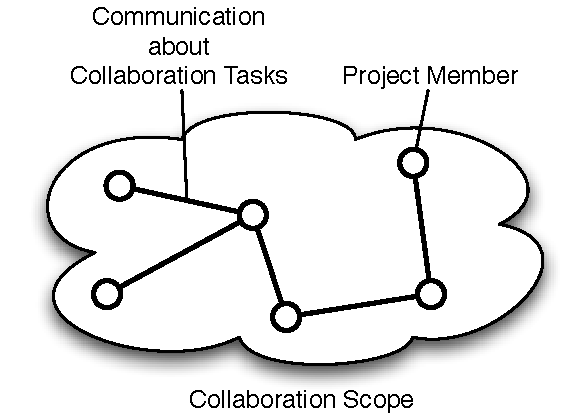
\includegraphics[width=8.0cm]{./figures/concepts}
% \label{fig:concept}
% \caption{Concept Visualization}
% \end{center}
% \end{figure}

\begin{figure*}[t!]
\begin{center}
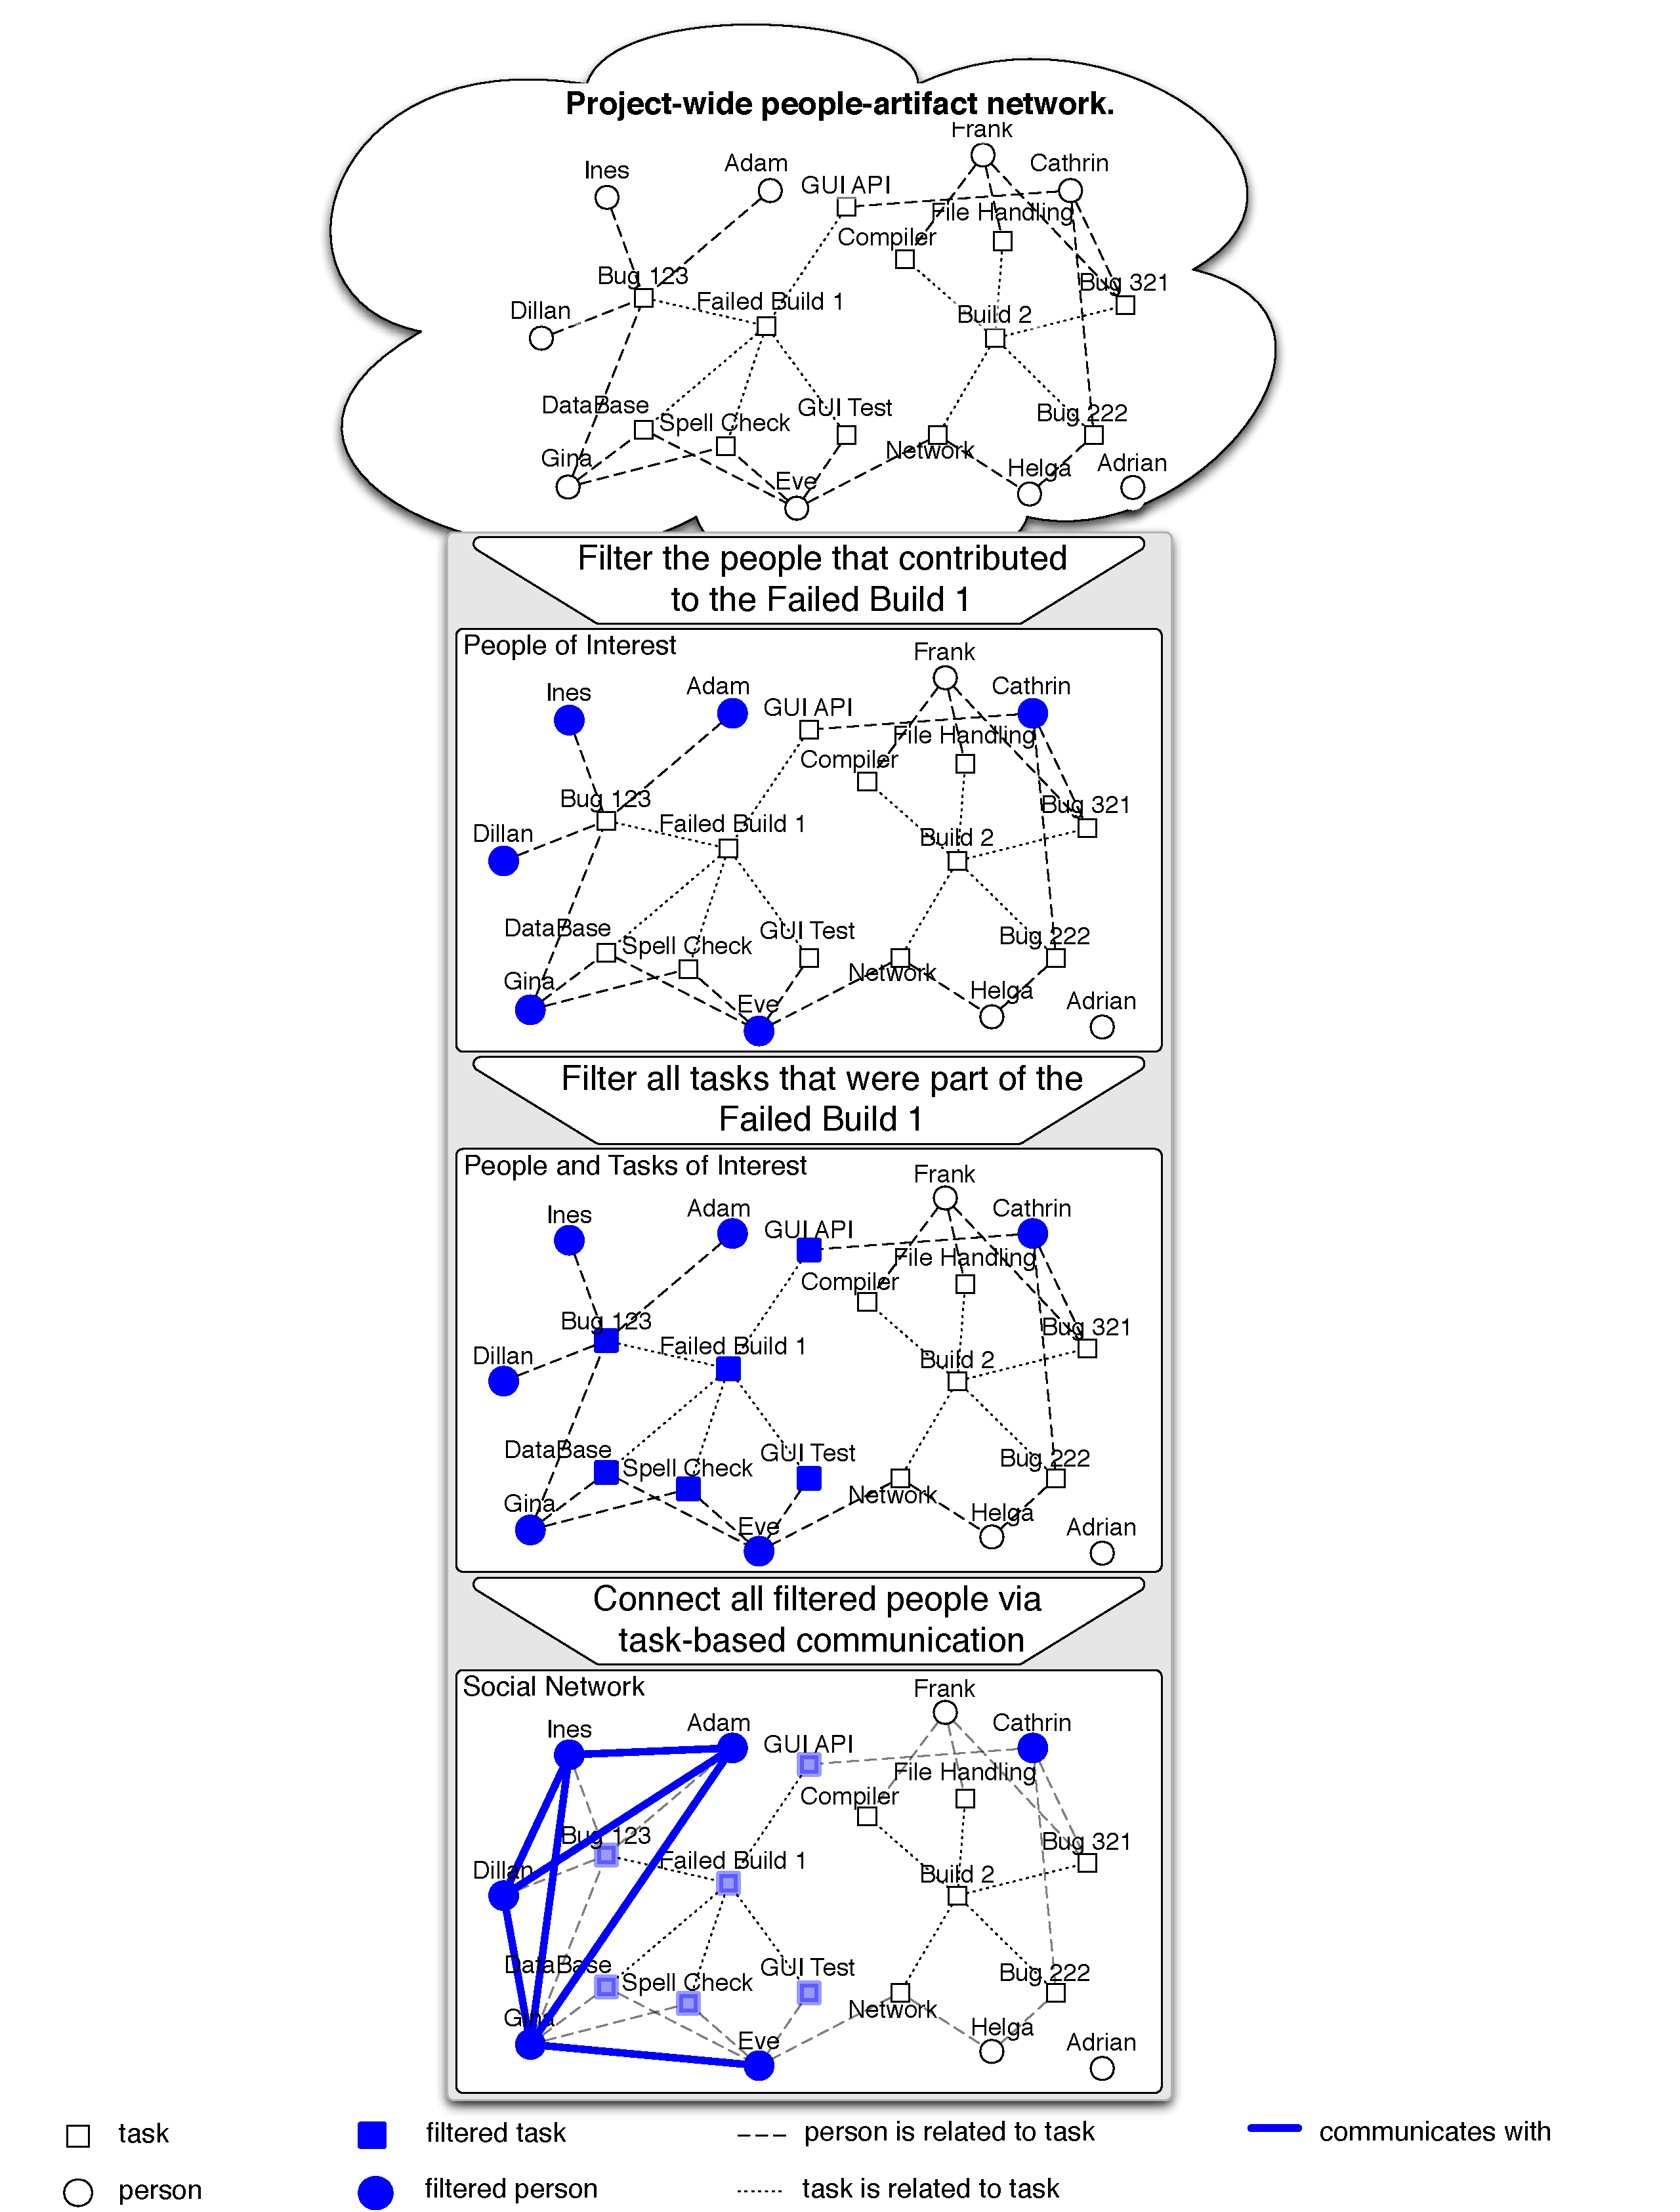
\includegraphics[height=0.9465\textheight]{./figures/grand_figure}
\caption{Social network construction examples in our approach}
\label{fig:network}
\end{center}
\end{figure*}

\subsection{Constructing Social Networks:}
The following three steps are used to construct a social network within a
collaboration scope: filtering of project members to identify nodes in the
network, filtering collaborative tasks to use as the context for collaboration,
and connecting project members to identify edges in the network. Each filtering
step includes criteria and reduces the set of \people s or \cu s from the entire
project. After collaborative tasks and team members are filtered, recorded
task-related communication is used to connect the nodes in the social network.

\paragraph{Filtering Project Members:}
To determine the set of nodes to be included in the social network we identify
those \people s that meet the criteria specified in the collaboration scope. In
our example, we restrict the team members to those who contributed to the failed
build, such as Adam, Eve, and Cathrin (coloured blue in Figure
\ref{fig:JazzProjectSN}). In addition, other constraints, such as temporal
% R2.1
constraints on when team members communicated about a task, can be added to
further reduce the included set of \people s.

\paragraph{Filtering Collaborative Tasks:}
Similar to the filtering of \people s, we use the criteria from the collaboration
scope to select \cu s. The \cu s provide the communication context used to
connect \people s in the following step. In our example, we restrict the tasks to
those included in Failed Build 1, such as GUI API, Bug 123, and GUI Test. The
filtering criteria can be based on properties of \cu s, such as task priority or
assigned team. Again, temporal constraints are often useful criteria, such as
selecting all development tasks contributed since the last build.

\paragraph{Connecting Project Members}
To connect \people s, creating edges in the social network, we leverage recorded
communication between the \people s in the filtered \cu s. For example, Gina and
Ines have both commented on Bug 123 and so we create an edge between them in the
social network. Our approach to constructing task-based social networks also
enables the inclusion of directed and weighted edges. Directed edges can
represent the direction of communication such as email sent from one team member
to another. Weighted edges can be used to represent the volume of communication
such as the number of emails sent.

\paragraph{}
While the filtering steps are independent, the order in which they are applied
can affect the composition of nodes and edges in the resulting social network.

\subsection{A Second Example -- Communication Brokers}
Here we provide a second example, applying project member and task filters in a
different order with differing criteria. This example demonstrates how social
networks can be used to find communication brokers between two project members.
This example is illustrated in the right column of Figure \ref{fig:network}.

Suppose, again, that you are the manager of a software team. Helga, a developer
in your project, complains that she needs information from Adam, but Adam has not
responded to information requests. Helga needs this information to complete her
work on Bug 222. You suspect that, due to time zone differences between
offices, Helga and Adam are rarely working at the same time and have trouble
communicating effectively. Social network analysis can identify other people in
the project that may be able to broker communication between Helga and Adam.

To construct a social network for this application, we filter the collaborative
tasks in the project keeping all tasks (coloured green in the right column of
Figure \ref{fig:network}). Then we filter the project members, keeping those that
have contributed to those collaborative tasks. Finally, using the recorded
task-based communication, we connect the project members to create a social
network for the entire project. By visualizing this social network we see that
Gina and/or Eve are good candidates to broker communication between Helga and
Adam. Choosing to use either Gina or Eve as a communication broker could be done
based on their geographic location with respect to Adam.

\paragraph{}
These two examples illustrate how the same repository could be mined for two
different collaboration scopes of interest to construct two different social
networks. An overview of software repository mining approaches to generate
developer networks are outlined in the Constructing Developer Networks sidebar.




\begin{figure*}[t!]
\begin{center}
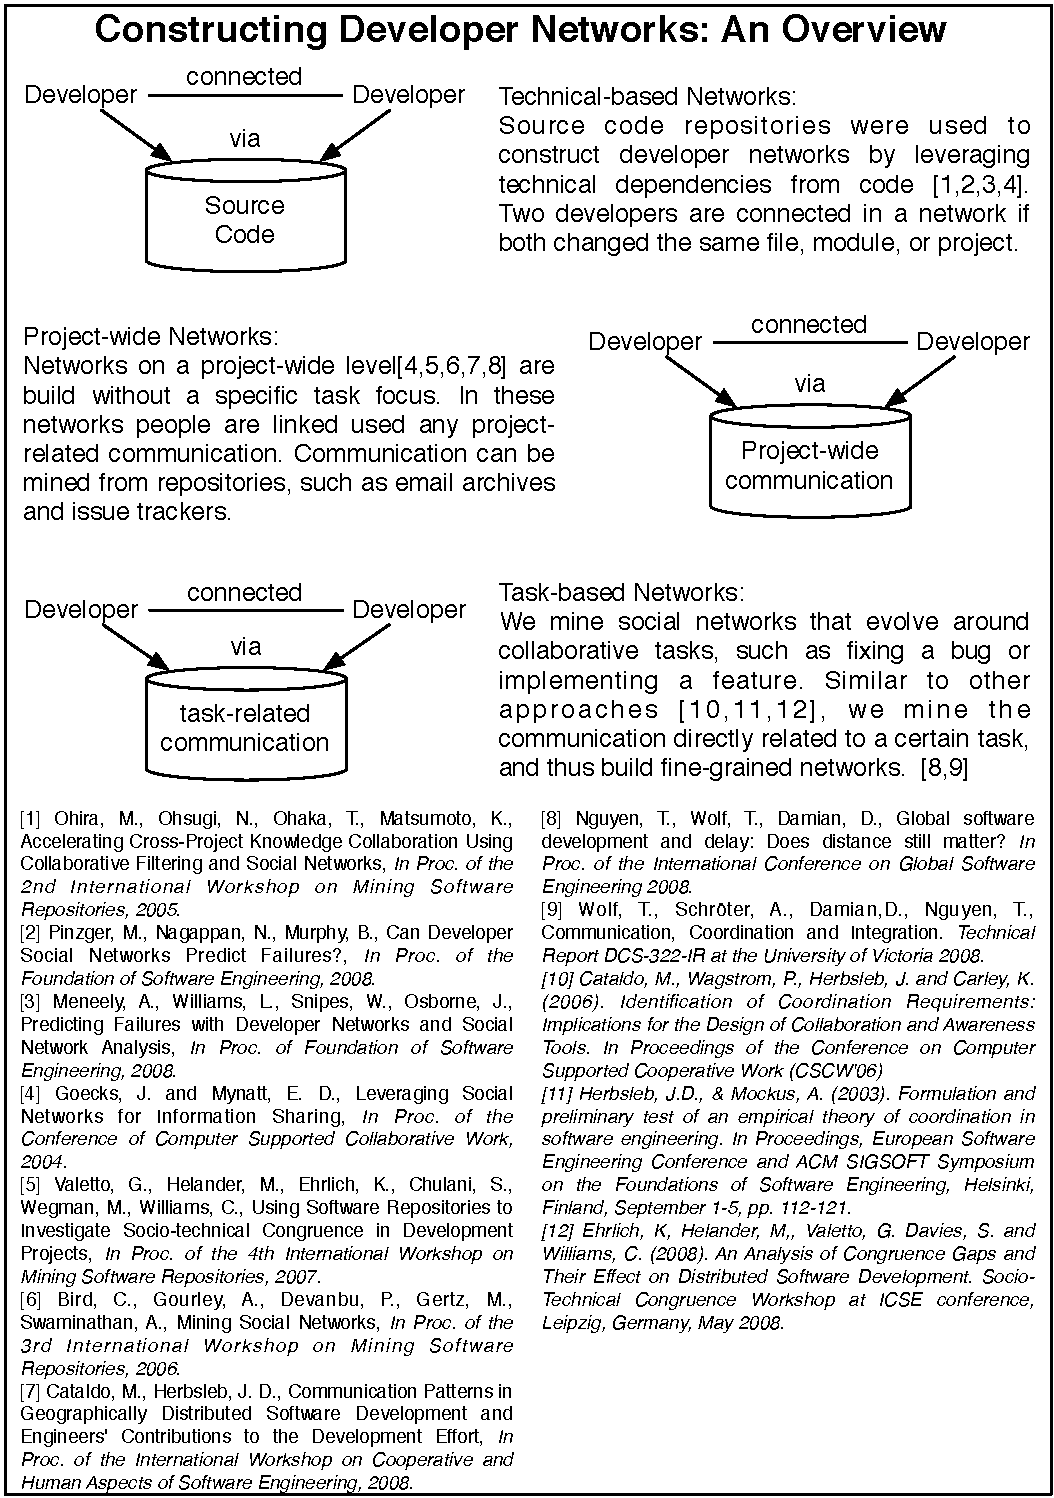
\includegraphics[width=0.7\textwidth]{figures/related_work.pdf}
%\caption{Constructing social networks}
%\label{fig:indep}
\end{center}
\end{figure*}



%[Some intro of Jazz repository]

% Commenting on work items is the main task-related communication and collaboration
% channel used by \jazztm\ developers. Work items represent single
% assignable and traceable tasks and a set of work items defines the tasks for each
% team in each iteration. Different types of work items represent defects,
% enhancements, user stories, and general tasks. The work items are assigned to,
% and owned by, project participants. The coordination that is necessary for the
% implementation of the work items is facilitated by work item collaboration
% behavior that includes contributors to comment or observe the communication
% around work items, by being subscribers to the work item.

\section{Social Network Analysis with \jazztm}

We applied our approach to mine and construct social networks with the IBM
Rational \jazztm\ project in several research studies. First, we describe how
\jazztm\ concepts and artifacts were mapped to the concepts used in our general
approach. Then, we describe our data mining tools, followed by two research
studies conducted using data extracted from the \jazztm\ development project.

IBM Rational is building \jazztm\ \cite{frost:ieeesoftware:2007} as a scalable and
extensible team collaboration platform for integrating development work across
task, build, source code, and planning management activities. \jazztm\ is
developed by a globally distributed team that uses \jazztm\ to manage its own
work. The \jazztm\ platform uses a client-server architecture, where the server
is the central data repository that stores data for \jazztm\ components. The
repository is accessible using a web-based client interface or an Eclipse-based
client. Our elements for constructing social network map to Jazz artifacts as
follows:

\begin{description}
\item[Project Members] are \emph{contributors} in Jazz.
Personal information, such as the name and email address of each contributor, as well as
project related information, such as team affiliations are available.

\item[Collaborative Tasks] are \emph{work items} in Jazz. Work items represent
the basic unit of work in \jazztm\ and can describe many types of tasks such as
bug reports, modification requests, or development tasks. Work items have a
comment-based conversation, a list of observing subscribers, and other attributes
such as, a creation date, a description, and an owner.

\item[Task-related Communication] is \emph{comments} on work items in Jazz.
Reading and writing comments on work items is the main collaboration mechanism in
Jazz as developers use comments to debate and discuss decisions. A thread of
comments forms a conversation that is attached the work item. Each comment
has a creation date, comment text, and an authoring contributor.

\end{description}

% XXX -- fix my location
\begin{figure*}[tb]
\begin{center}
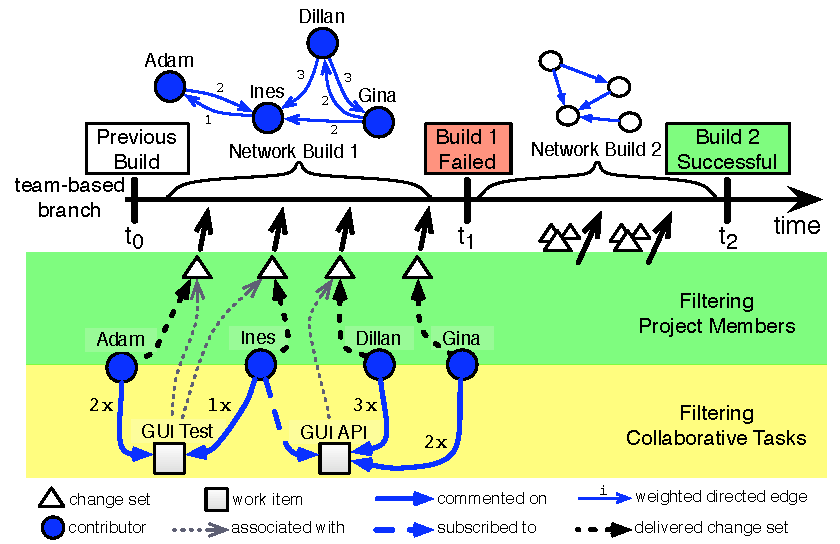
\includegraphics[width=1.3\columnwidth]{./figures/BuildResultNetworks}
\caption{Construction of social networks for build failure prediction}
\label{fig:BuildSNs}
\end{center}
\end{figure*}

\subsection{Data Mining Tools for \jazztm}
In order to extract the elements needed to construct and analyze social networks,
we implemented several data mining and social network analysis tools. To extract
data of interest, we developed a plug-in for the Eclipse-based \jazztm\ client
that used the provided Java API to query and retrieve the desired data from the
repository.

The \jazztm\ development project has a large \jazztm-based repository containing
more than 40,000 work items, 150 contributors, and 5,000 build results. We
needed to collect data from the live development repository without affecting the
\jazztm\ development team's server performance, potentially disrupting their
work. To meet this goal, we designed our data extraction tool to be minimally
invasive and to use incremental queries, extracting small portions of the data
set at a time, to minimize performance degradation.

Further, the querying and processing of the extracted data to construct social
networks is an additional challenge because it is data and time intensive. For
example, extracting and processing all work items from the repository took
several hours. Thus, it is not feasible to extract and process all of the
information needed to construct social networks in real-time. For this reason, we
import the data of interest into a reporting and analysis database. This approach
allowed us to use a large proportion of the data in the \jazztm\ team's
repository for social network construction and analysis without adversely
affecting their development environment.

% Each data type's external XML file representation is independent so that a single
% query result can already be used for analysis, without requiring all associated
% data types or associations. For example, when only exporting the work items that
% were created or modified during a specific week, the resulting data file can
% already be analysed without the need of any associated data types like the
% contributors. In addition, data and associations between data types that result
% from subsequent queries can be added without changing the previous extracted
% information. This data structure enables us to mine large data sets in many small
% through incremental queries without affecting the Jazz server repository.

To process the data from the database we used the Java Universal Network/Graph
Framework (JUNG) to construct and visualize the task-based social networks and to
compute social network analysis measures. Our tools also generate data sets for
use as inputs to other tools, such as statistical analysis using the R language,
or social network analysis using UCINET.

%\paragraph{Filter Project Members}
%\ \\
%In \jazztm\ we filter \people s by different criteria to focus on people to meet
%each collaboration scope. One way to do that would be to focus on all people that
%made changes to the source code included in a build. For that we would identify
%all chances made for that build and identify the people that made those changes.

%\paragraph{Filter Collaboration Tasks}
%\ \\
%One major task during the \jazztm\ development would be to deliver a successful
%build of \jazztm. Our XXX would focus on a build within \jazztm\ and only include
%work items that are build related. In addition, the XXX would define the time
%frame starting on the previous build and the build of interest.

%\paragraph{Connect Project Members}
%\ \\
%Contributors comment on work items to ask questions, debate descisions, or to
%provide additional information, such as screenshots. A series of comments on a
%work item forms a conversation thread. When connecting \people s while
%constructing our social networks, we connect those who have commented on a work
%item, as we assume that they have exchanged information and thus communicated.
%Additionally, we assume that subscribers of a work item listen to the
%communication, but have not actively contributed. We also include the creator of
%the work item as a contributor because a work item's initial description is the
%start of the conversation.

% The communication between two \people s is directed, since participating in a
% work item conversation thread means sending and receiving information. Whereas,
% subscribing to a work item only provides one-way communication, so directed edges
% are used to connect \people s. Weights can also be applied to communication links
%  by using the number of comments exchanged between two \people.


\subsection{Research Studies Using Social Network Analysis}
We used the mined task-based social networks in two of our research studies that
map to the more general build failure \cite{wolf:tr2008} and communication
broker \cite{Nguyen:2008Distance} examples provided earlier.

\paragraph{Communication Structures to Predict Build Failures}
\ \\
In this study we were interested in investigating whether properties of an
integration team's social network have any relationship with the integration
outcome. Code integrations (referred  to  as builds in Jazz)  are frequent and
very important in the Jazz project. The continuous integration process requires
regular daily and weekly integrations of each team's work into an assembled
product. A build can succeed or fail due to compilation, testing, or other
integration errors.

To integrate in \jazztm, the members of a development team commit source code
changes (change sets) to a team-based branch. Each change set is associated with
the work item that describes the change it implements, and contributors comment
on the work items to discuss the changes. As such, the \emph{collaboration scope}
of this study is the communication of contributors who have delivered change sets
that were included in each build. 

%DD. Shortened the text to avoid repeition from section 1, as per comment #2

To construct the social networks for Build 1 at time t$_1$ (as illustrated in
Figure~\ref{fig:BuildSNs}), we followed the steps outlined in our Failed Build
example described earlier: we filtered the contributors that delivered change
sets between t$_0$ and t$_1$ and identified all work items that were associated
with code change sets in Build 1. To connect contributors in the social network
we add a directed edge between each pair of contributors who have either
commented or subscribed to a common work item since the last build. The weight on
directed edges represents the number of comments on the shared work items.

% T.W. Changed the following paragraph to address point 3 from revision 2
After we constructed the social networks for each integration build of the five
teams
% R3.2
(between 48 and 60 builds for each team), we computed different social network
measurements, such as \emph{centrality}, \emph{betweenness}, and
\emph{density}~\cite{Wasserman:1994dz} and investigated their relationship to
integration outcomes. Although none of these measures can independently predict
the build outcome, when used in combination they are more powerful. We developed
a predictive model by training a
% R2.4
Bayesian classifier that was able to accurately predict failed build results. The
recall and precision values of the predictions using measures of social network
structure is shown in Table~\ref{tab:predictionResults} for the five teams.
% R3.2
In order to validate our model for each of the five teams we used \emph{leave one
out cross validation}, which trains a model for each set of data points that is
in size one smaller then the full set, and then predicts the data point that is
not in the training set. Study details are available in technical
report~\cite{wolf:tr2008}.


\begin{table}
\small
\begin{tabular}{r|c c c c c|c}
\hline
  & \multicolumn{5}{c|}{Teams} & Std.Dev. \\ \hline
Recall 		& 55\% & 75\% & 62\% & 66\% & 74\% & 8.38\% \\ 
Precision 	& 52\% & 50\% & 75\% & 76\% & 66\% & 1.34\% \\ \hline
\end{tabular}
\caption{Prediction results for the five teams}
\label{tab:predictionResults}
\end{table}



% R2.4 NOTE FROM DANA: NO NEED TO HAVE THIS NEXT PARA, SO I COMMENTED IT. THE
% REVIEWER WAS JUST BEING VERY TOUGH.. 
% Although, the results are compared to a general failure probability of 50\%, we
% consider this result as a first step towards indicating that communication
% influence source code quality.


\paragraph{Communication Structures in a Large Distributed Project}
\ \\
In this second study \cite{Nguyen:2008Distance} we were interested in the
project-wide communication structure of the geographically distributed \jazztm\
development team. A quantitative analysis of response time for task
communication and task resolution times revealed a lower than expected impact of distance on these
factors. We explored the project's social networks for useful insights that might
explain this effect. Specifically, we were interested in identifying properties
of the social networks, such as cohesiveness of the distributed teams, that were
related to the results of communication delay and distributed collaboration.

The \emph{collaboration scope} of this study is the entire project, and thus
includes all collaborative tasks, and all contributing project members. In this
case, connecting project members is the key step to create a project-wide social
network. 

%DD shortened the text to address comment #2. 
To construct the project-wide social network we followed the steps as
exemplified in Section 1.3 (the communication broker example).


The resulting social network is illustrated in Figure~\ref{fig:JazzProjectSN} in
which ovals indicate the teams at each geographic site. We used the \emph{k-core}
and \emph{core-periphery} tests \cite{Wasserman:1994dz} to analyze the properties
of the network structure. These tests allowed us to test whether multiple
cores can be identified in the network, or the network shows a star-like 
structure in which a single core mediates communication with the developers on
the periphery of the network.
%R3.5 && R2.5

The results indicate that the project-wide team collaborates as a cohesive team
with one large core, as opposed to many loosely connected clusters. The colors in
the figure illustrate how close a team member is to the core of the whole
project. In red we show a core of active developers (60 of
112 project members) where each developer
communicates with at least other 25 developers from the core. The other
colors, from yellow to light blue, indicate different lower degrees of communication in
the project. Further, using the
\emph{group degree centrality} \cite{Wasserman:1994dz} measure, we also found
that each geographic location has roughly equal centrality and used the people in
the core to stay connected to the rest of the large team. This means that project
members communicate well with project members at each other geographic location.
This may explain why distance had an insignificant effect on communication response
and task resolution time in the large distributed team.

% R3.2
In summary, we learned from this study that communication delay as a result of
distribution in global teams can be overcome with recent
collaboration tools and practices. From our experience with the Jazz team, best practices such as prioritizing
off site requests and tools that integrate development, project
management and communication play a major role in achieving these results.

\begin{figure}[t]
\begin{center}
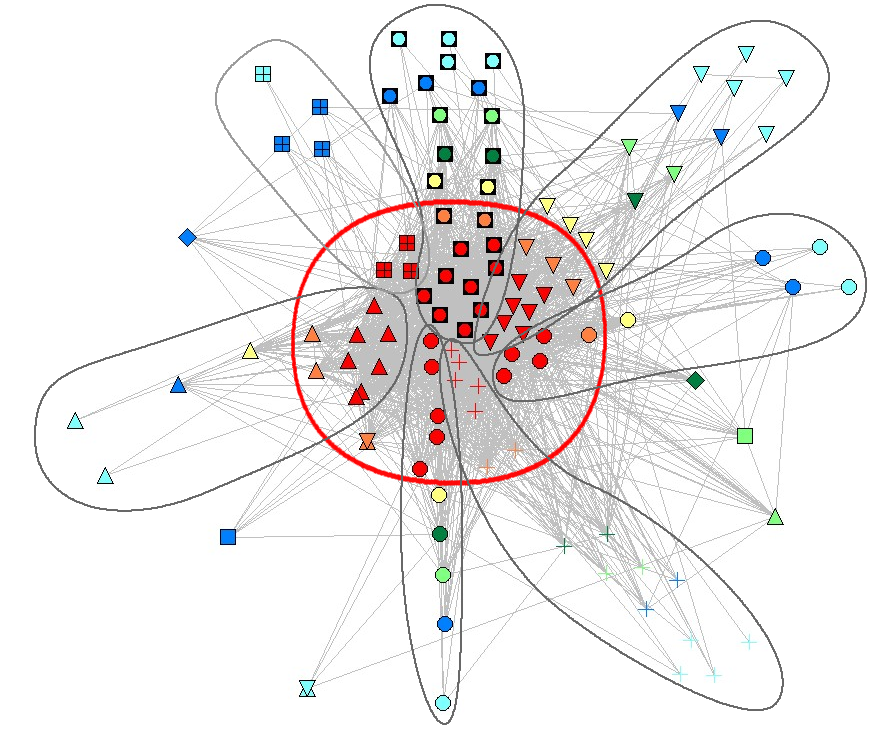
\includegraphics[width=0.99\columnwidth]{./figures/JazzProjectSN}
\caption{Project-wide communication-based social network}
\label{fig:JazzProjectSN}
\end{center}
\end{figure}

% ~\cite{Seidman:1983sn}
 % ~\cite{Borgatti:2000kl}
% ~\cite{Everett:2005dn} Details are published






\section{Practical Implications for Deployment} 
% [How to integrated our approach in the used repositories and tools to support
% project during development?]

Our approach to mining and constructing social networks, as well as the results
of our studies, have several implications for software practitioners.

\paragraph{Scalable Mining and Analysis Tools}
\ \\
By incrementally mining and using a secondary reporting database (or data
warehouse), we can reduce load and performance problems on the mined software
repositories. Our approach is useful for practitioners who must not impact the
performance of their team's repositories.
% R3.3
This has been proven useful during our extraction of information from the Jazz
repository, which was under constant load due to the global distribution of the
more than 140 Jazz team members.
%
Extracted data, constructed networks, and network analysis measures can be stored
in the data warehouse to avoid extracting or recomputing them multiple times. For
example, the social network using the set of work items and communication around
each build can be stored in the data warehouse and is directly accessible for any
number of further analyses. Computationally intensive analysis and predictions
can be conducted using the data warehouse or by a client accessing the data
warehouse. Once task-based social networks and network analysis measures are
stored in a data warehouse, visualization of social networks and further analysis
becomes efficient and non-intrusive to the users of repositories.

% These networks and measures can assist developers, enabling task-awareness and
% expertise seeking. Additionally, team-leaders and managers can examine social networks and their computed measures
% in the context of project performance data such as integration outcomes.

\paragraph{Team Awareness through Social Network Visualization}
% \ \\ 
Developers working on interdependent tasks can benefit from the visualization of
the social network of the team members who contributed to the interdependent
tasks. The information in the network can include developer contact and
availability, as well as a list of other tasks that they are working on. This
information is particularly important for newcomers to a project, who lack
project specific expertise, such as who has been involved with a particular task,
or in architectural decisions.
% R3.3
We are currently conducting a case study to identify which information is
valuable to support developers and what visualization conveys them most
effectively.
 



% Collaboration scope  focusing on specific teams, inter-team communication, or
% specific task criteria.

\paragraph{Outcome Prediction Using Social Network Analysis}
\ \\
Another application for social network analysis is to predict project outcomes
such as build results based on information about team communication behaviour.
Practitioners can build tools that are embedded in the development environment
that inform developers about the health of upcoming builds. An awareness
notification system that uses a build failure prediction model could indicate
whether the current communication patterns are likely to result in a failed build. 

Building a predictive model from social networks constructed with data mined
from task and task-communication repositories could be done with the following
four steps:

% Note that the steps focus on the integration builds a a certain team and can be
% applied for all teams in parallel.

%\begin{enumerate}

%\item In frequent time intervals (e.g. 30 min.), the social network is
%constructed on the communication about the tasks that are associated with the
%source code changes that are made after the last build. The construction requires
%the querying of the main repositories. The social network measures are computed
%for the network and the resulting measurements and the network are stored and cached in
%the warehouse so that the subsequent network constructions only need to query the
%communication data from the last time interval (e.g. 30 min.).

%\item The trained predictive model that is stored in the warehouse and the
%computed network measurements are used to predict the result of the next upcoming
%build. The prediction result in the warehouse is accessed by the development
%environments to indicate the current prediction result to the developers.

%\item Whenever an integration build finished, an automated process queries the
%remaining new communication that occurred after the last network construction
%from step 2 and the time of the build. The final build related
%communication-based social network and its measurements are constructed, computed
%and stored in the warehouse. The process can either be triggered by notifications
%on subscription or by frequent look-ups.

%\item A new prediction model is trained on all build related networks and
%measurements that are stored in the warehouse. The trained model is stored in the
%warehouse and replaces the previously stored model. The data set that is used to
%train the prediction model increases with each new build and the predictions
%become more precise.
% 
%\end{enumerate}

% To build a predictive one needs to mine the social networks for each build in
% order to populate the data warehouse. All mined social networks of past builds and the associated
% build results are used to train a predictive model. Whereas the social network
% for the upcoming build is only stored in the warehouse for later predictions. 



\begin{enumerate}
\item \textbf{Initialization Predictive Models:}
Initialize the predictive model using the social networks and
outcomes for all existing builds. Store the data on social networks, build
outcomes, and predictive model in a data warehouse for later use.
\item \textbf{Construct Social Network for Upcoming Build:}
Construct the social network for the upcoming build as described
in our approach.
\item \textbf{Predict the Upcoming Build Outcome:}
Calculate network analysis measures for the constructed social
network and use them as input to the predictive model. The model then predicts
an outcome for the upcoming build. At this point, a manager could make
proactive adjustments to attempt to prevent a predicted build failure.
\item \textbf{Update Predictive Model:}
Finally, after the upcoming build has been completed, update the predictive
model to include the social network, network measures, and outcome of the latest
build. The model can then be used again to make an outcome prediction for the
next upcoming build (starting with Step 2).
\end{enumerate}

% Note that steps 2 and 3 are executed repeatedly and only interrupted when a build
% is done in step 4.

%This repository mining and model building approach using task-based
%communication can also be applied to predicting other project-related variables
% such as post-release defects or iteration scheduling accuracy.

If the system indicates a build failure, further analysis could
identify communication deficiencies and prompt managers to rectify the problem
before the build occurs, as described next.
% R3.3
% We are currently conducting a case study to identify how the predictions are
% used by the Jazz team.


\paragraph{Effective Management through Social Network Analysis}
% \ \\

%R0 and R2.6
Beyond visualizations, computed social network measures can be used
by
management as an aid in preventing failed builds. Our research shows that the quality of
communication does matter in the quality of integrations. Monitoring and
affecting communication behavior is a strategy to prevent failures. Software
engineers differ in the expertise and knowledge they bring to collaborative tasks. Team
performance depends not only the information available to developers and the
distribution of knowledge within the team, but also on the communication
structure that facilitates knowledge dissemination within the team. Although we
have no evidence that individual measures of communication structure can
predict integration failure, these measures can be used in identifying
problematic communication behavior likely to result in failed integrations.
Actions that management can take to prevent failures for a
particular team include:

\begin{enumerate}
\item \textbf{Compute Social Network measures or Run Predictive Model early in
the project:} In our study of Jazz, the predictive model performed well even
with the first 25\% of the team communication data (i.e. first quarter of
project timeline). If this is true in other development environments,
practitioners should use this information very early in the project. If the
model predicts error, see next step. Otherwise, computing social network measures such as
density, betweeness and centrality early in the project is an alternative
option that could signal problematic communication behavior in the project.
\item \textbf{Examine team communication structure:}
Identify the presence of patterns of communication that can, when analyzed in
light of project specific technical dependencies, be problematic. An example of
problematic communication structure indicated by social network
measures is that of a team with high coordination needs before an integration
but with a communication network of low density. It is possible that there are too many missing communication links between developers that have
technical dependencies~\cite{ehrlich2008:gaps}, or
there is an overall lack of communication in the team. Another example is of a team with several
distributed subteams that need to coordinate and in which a number of
developers have high betweeness but the subteams themselves have little
communication across distance. This may indicate that there are
clusters of developers who should communicate directly, and that
the subteams are only loosely connected and have communication brokers that
may become bottlenecks. 
\item \textbf{Improve communication or knowledge management
procedures:} Adjust communication and knowledge management processes or tools in
the project, to address specific situations identified at previous step. 
If communication links between developers with
coordination needs are missing, assigning communication brokers so that
these developers can better coordinate interdependent work is an
option. Equally valuable, increasing the awareness of these coordination needs
as well as developers' expertise areas in the current project could be done
through regular project meetings or more adequate documentation of these dependencies in project specific knowledge repositories. In other situations, if
communication across distances is relying on information brokers, managers
should consider supporting alternate points of contact in the clusters
identified as relying on these brokers, or enforce documentation of information
that becomes available to everyone in the project. Both these options help
mitigate the risk of information brokers becoming unavailable in the project. 
\end{enumerate}

Despite our intention to be as specific as possible, these 
recommendations for action should consider and be applied in the
particular context of each project. Managers should use the
insights obtained from the examination of communication structures in their
project as a starting point in their further analysis of 
communication in relation to the particular technical and
organizational characteristics of their project.




% Using social network measures, one can
% detect the presence of communication clusters in a distributed project, or
% dysfunctional behavior, such as a lack of communication activity around a
% critical task for an upcoming release.

% On a regular basis, the measures can be reported automatically for the
% project-wide communication network or for specific collaboration scopes. For
% example, this focus can be on tasks related to specific activities (e.g.,
% requirements analysis or maintenance), or certain task properties (e.g., tasks
% within a time range, with high priority, or assigned to one team). Managers and
% team leads monitoring these reports can then maintain awareness of the
% communication structures and possible sources of communication problems within
% these contexts. Detecting problematic communication structures, such as loosely
% connected teams where brokers may become bottlenecks enables project leaders to
% take action and adjust communication processes in a timely and proactive manner.




% \section{Related Work} The related work consists of three parts. The first is
% focused on how social network were build in the past. The second shows practical
% applications that make use of social networks and the third part gives a quick
% overview over  what has been done with regards to failure prediction.
% 
% \subsection{How To Build Social Networks} Most automatically constructed social
% networks are mined from SCM's~\cite{msr07:weissgerber,msr04:lopez,fse08:pinziger,
% fse08:meneely}. These approaches usually assume that two
% developers that worked together on a module are connected. In this case working
% means that they changed the same module within a pre defined timeframe. This has
% of course the disadvantage that the project specific communication between
% developers is missing. One way to capture part of this communication is to mine
% e-mail archives~\cite{bird:msr:2006,fse08:bird}. Still this medium is incomplete with
% respect to actual ongoing communication therefore we leverage the discussion
% around work items as provided within \jazztm\. But where were such social networks
% used?
% 
% \subsection{Practical Applications for Social Networks} Social network have been
% used in many different ways. Recent research has manly focused on knowledge
% distribution and failure prediction.
% \begin{description}
% \item[Knowledge.] Efficiently distributing knowledge and fostering awareness in
% teams is a hot topic within software development.
% Several studies have addressed this issue recently. They reach from expertise
% recommending systems within \cite{msr07:minto} and across projects \cite{msr05:ohira}.
% \item[Prediction.] Other studies have leveraged simple networks mined from SCM's
% to predict the existence of post release failures in software modules like
% binaries~\cite{fse08:pinziger,fse08:meneely}.
% \end{description}
% Of course there are more than these application like ... argued the congruence of
% social and technical networks is of use for It governance and de Souza used
% social networks to study the behavior of teams with respect to whom they need and
% want to display their actions.
% 
% \subsection{Failure Predictions} Recent research mostly focused on predicting
% whether a software module (e.g. files or binaries) will fail after shipping a
% product. Most features used to predict this kind of failures leverages the
% technical part like module dependencies, code changes or simply code complexity.
% One of the more recent prediction models by Zimmermann and Nagappan uses social
% network measures on module dependency graphs to predict if a module is
% failure-prone~\cite{icse08:zimmermann}. Others leveraged organizational structures
% evolved around software modules. They connected those modules via developers that
% worked on them to the organizational structure~\cite{icse08:nagappan}. There have been
% studies that go one step further and do not focus on organizational structures
% but look at how developers are connected, mainly those studies like ... and ...
% constructed their networks from SCM systems. These networks connect developers
% through modules they worked on together, which of course misses every other
% communication that went on during that time.
% 
% All in all those approaches focus on failures that will occur after the release
% of a software product since those are most inconvenient for the end user. In
% contrast to that we focus on the product quality during the development. In
% particular on the outcome of builds since if your build does not satisfies the
% minimum quality requirements or does not even build than you cannot ship the
% product. Kim et al. had a similar approach which is more fine grained. They
% predicted if a change introduces a failure into the software \cite{icse07:kim}. This
% method can be used during development but the fine level of detail does not focus
% on the important part namely predicting if you reached a deployable state or not.




\section{Conclusions}
Task-based social network mining and analysis enables you, as a participant in a
software project, to tap into a vast pool of otherwise inaccessible communication
information. Our approach has been applied to two scenarios with the Jazz project
illustrating its applicability and gleaning new insights into the social patterns
of that team. The use of social networks in software engineering is relatively
unexplored and holds much promise for future applications.

%  Mining repositories and social networks gained focus by researchers to analyze
% software development projects and the involved technical and human
% relationships. While researchers published impressive findings, few of the
% techniques are integrated and used in the development environment to directly
% support the project. We provide an approach of mining task-related
% communication-based social networks for any repositories that support \people
% s, \cu s, and communication. The feasibility of the approach is shown by two
% studies mining the Jazz repository of the Jazz development project. We propose
% to utilize social network analysis to directly support the mined project. A
% variety of practical applications in the area of reporting or awareness
% applications can support the daily work of project participants by integrating
% the mining process into the development environment. We propose initial steps
% to realize the integration without affecting the performance of the main
% repositories used.